\chapter{Building the groundwater model}\label{ch:c3}
Raven's HRUs are irregular areas; MODFLOW needs a regular three-dimensional grid. This chapter follows the model builder step by step. It shows which HRUs are coupled, how their polygons are placed on a map
and covered with a grid, and how much of each HRU falls in each cell. It then shows how the layers are built from the land
surface down to bedrock, which MODFLOW files are written, and how MODFLOW solves each step.

\section{From HRUs to a groundwater grid}\label{ch:grid}
\subsection{Which HRUs are coupled}
An HRU is \emph{coupled} when its \cmd{AQUIFER\_PROFILE} in the \cmd{.rvh} file names a profile defined in the
\cmd{.rvp} file. HRUs with \cmd{[NONE]} (or an empty entry) keep Raven's usual behaviour. Disabled HRUs are never
coupled (Raven prints a warning). We write $\mathcal{K}$ for the set of coupled HRUs and $p(k)$ for the profile of HRU $k$.

Raven checks two rules at start-up:
\begin{itemize}
\item No Raven process may take water \emph{out of} \cmd{GROUNDWATER} in a coupled HRU (MODFLOW owns that water);
Raven stops with an error naming the process.
\item If a process sends water \emph{into} \cmd{GROUNDWATER} in an \emph{uncoupled} HRU, that water leaves the model;
Raven warns so the user can restrict the process with \cmd{:-->Conditional}.
\end{itemize}

\subsection{Map projection}
The HRU polygons are read from a GeoJSON file. GeoJSON coordinates are longitude $\lambda$ and latitude $\phi$ in
degrees, which cannot be used directly for areas and distances. Raven converts them to metres with the
\emph{Lambert azimuthal equal-area} projection \cite{snyder1987map}, centred on the average centroid
$(\lambda_0,\phi_0)$ of the coupled HRUs, on a sphere of radius $R=6\,371\,007.181$ m:
\begin{align}
k' &= \sqrt{\frac{2}{1+\sin\phi_0\sin\phi+\cos\phi_0\cos\phi\cos(\lambda-\lambda_0)}},\\
x &= R\,k'\cos\phi\,\sin(\lambda-\lambda_0),\\
y &= R\,k'\left[\cos\phi_0\sin\phi-\sin\phi_0\cos\phi\cos(\lambda-\lambda_0)\right].
\end{align}
The reverse conversion (used to look up map values at cell locations) is
\begin{align}
\rho&=\sqrt{x^2+y^2},\qquad c=2\arcsin\frac{\rho}{2R},\\
\phi&=\arcsin\!\left(\cos c\sin\phi_0+\frac{y\sin c\cos\phi_0}{\rho}\right),\\
\lambda&=\lambda_0+\operatorname{atan2}\!\left(x\sin c,\;\rho\cos\phi_0\cos c-y\sin\phi_0\sin c\right).
\end{align}
\begin{plain}
This projection keeps areas correct, which is what matters for water volumes: one square kilometre on the map is one
square kilometre on the ground, anywhere in the model area.
\end{plain}

\subsection{The grid}
By default a square grid with cell size $\Delta$ (\cmd{:GridCellSize}, default 1\,000 m) covers the rectangle around all
coupled HRUs. Rows are numbered from north to south and columns from west to east. The plan-view cell (a whole column of
layers) is indexed $i$; its lower-left corner is $(x_0+c\Delta,\;y_0+(n_r-1-r)\Delta)$ for row $r$ and column $c$. Rotated
grids, grids refined around rivers and wells, quadtree grids, meshes that follow HRU boundaries and imported cells are
described in Section~\ref{sec:gridtypes}; everything below applies to all of them, with cell $i$ a polygon of area $A_i$.

\subsection{Polygon areas}
The area of a polygon with corners $(x_1,y_1),\dots,(x_n,y_n)$ is given by the shoelace formula
\begin{equation}
A=\tfrac12\sum_{j=1}^{n}\left(x_jy_{j+1}-x_{j+1}y_j\right),\qquad (x_{n+1},y_{n+1})=(x_1,y_1).
\end{equation}
The result is positive when the corners run counter-clockwise. Raven orients outer boundaries counter-clockwise and
holes clockwise, so the area of a polygon with holes is simply the sum over all its rings.
\begin{example}[: shoelace formula]
A square from $(0,0)$ to $(2,2)$ km: $\tfrac12[(0\cdot0-2\cdot0)+(2\cdot2-2\cdot0)+(2\cdot2-0\cdot2)+(0\cdot0-0\cdot2)]=\tfrac12(0+4+4+0)=4$ km$^2$.
\end{example}

\subsection{How much of each HRU lies in each cell}\label{sec:linkage}
For every HRU polygon $P_k$ and every cell $\Omega_i$ it touches, Raven cuts the polygon to the cell rectangle with
the Sutherland--Hodgman clipping algorithm \cite{sutherland1974clip} and measures the area of what remains:
\begin{equation}
A_{k,i}=\left|P_k\cap\Omega_i\right| .
\end{equation}
For rectangular cells (regular and quadtree grids) the polygon is clipped by the cell rectangle; for convex cells (HRU
meshes) by the cell polygon; a concave imported cell is split into triangles and clipped by each. The clipping works one
cell edge at a time: walking around the polygon, it keeps the corners that are inside the edge
and adds a new corner wherever the polygon crosses the edge. After four edges, what is left is the part of the polygon
inside the cell; the shoelace formula gives its area. (This gives the correct area even for concave polygons.)

\begin{example}[: overlap areas]
An HRU of 10 km$^2$ lies over three 2~km cells, covering 4.0, 3.5 and 2.5 km$^2$ of them. Its overlaps are
$A_{k,1}=4.0$, $A_{k,2}=3.5$, $A_{k,3}=2.5$ km$^2$, and the fractions of the HRU in each cell are 0.40, 0.35 and 0.25.
Every flow from this HRU to the grid is split 40/35/25.
\end{example}

\subsection{Active cells and their profile}
A column is \emph{active} when the coupled HRUs cover at least a fraction $f_{\min}$ (\cmd{:MinCellCoverage}, default
0.25) of it:
\begin{equation}
a_i=\sum_{k\in\mathcal{K}}A_{k,i}\ \ge\ f_{\min}\,\Delta^2 .
\end{equation}
An active column takes the profile of the HRU with the largest overlap (the \emph{dominant} HRU),
$p(i)=p\!\left(\arg\max_k A_{k,i}\right)$. Fluxes still use the exact overlaps, so a column shared by two HRUs receives
water from both.

The table of overlaps $A_{k,i}$ over active columns is called the \emph{linkage}. It is the single source of truth for
moving water between HRUs and cells in both directions (Sections~\ref{ch:recharge}--\ref{ch:stores}).

\begin{watch}
The polygon area of an HRU need not equal its \cmd{AREA} in the \cmd{.rvh} file (Raven prints a warning when they
differ by more than 5\%). This does not break the water balance: volumes are always computed from the \cmd{.rvh} area
and split by overlap \emph{fractions}.
\end{watch}

\subsection{The linkage cache}
Computing the linkage requires reading and clipping every polygon. The result is saved in \cmd{<output>/mf6/linkage.cache}
(or the file named by \cmd{:LinkageCache}). The cache is labelled with a fingerprint (an FNV-1a hash) of the GeoJSON
file together with the ID field, the cell size and the list of coupled HRUs; if any of these change, Raven recomputes
the linkage. Numbers are written with 17 significant digits, so a run that reads the cache gives exactly the same
results as one that computed it.

\begin{figure}[!htbp]\centering
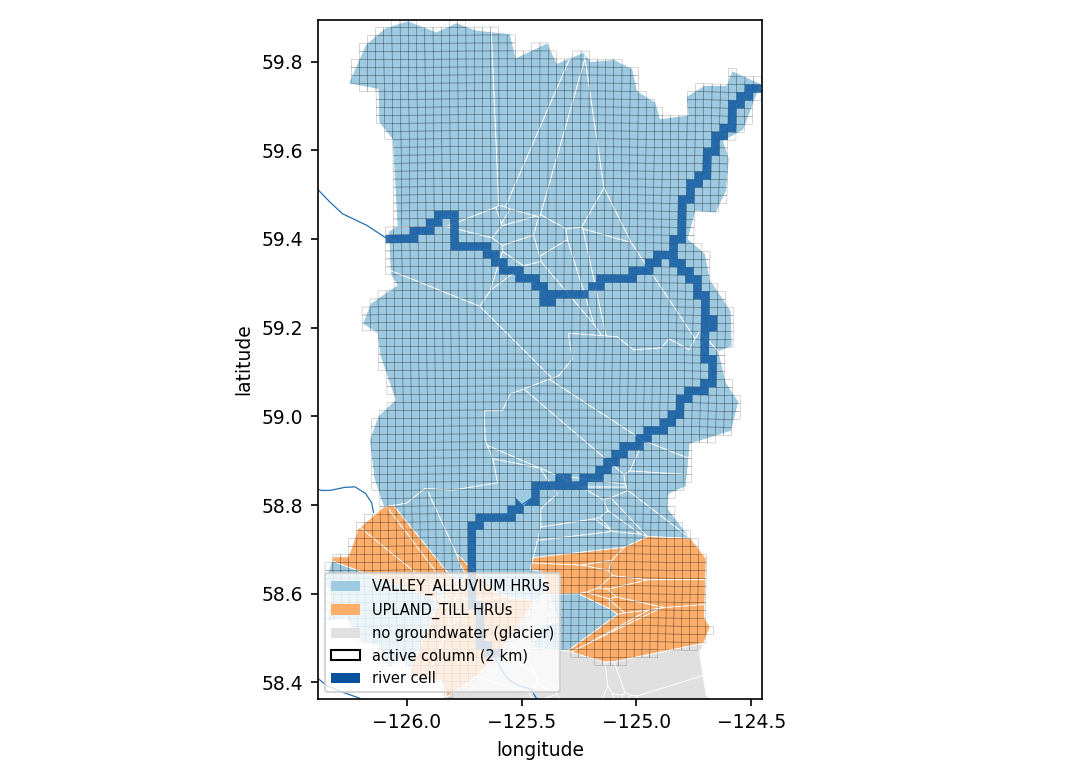
\includegraphics[width=0.9\linewidth]{figures/fig_grid_liard.png}
\caption{Liard example: coupled HRUs (colour = aquifer profile), active 2~km columns and river cells.}\label{fig:grid}
\end{figure}

\section{From one HRU to its cells: a complete example}
\begin{figure}[!htbp]\centering
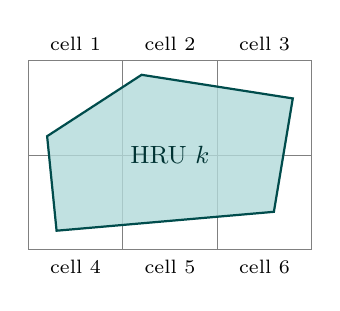
\begin{tikzpicture}[x=1.2cm,y=1.2cm]
\foreach \x in {0,1,2,3} \draw[gray] (\x,0) -- (\x,2);
\foreach \y in {0,1,2} \draw[gray] (0,\y) -- (3,\y);
\fill[teal!30,opacity=0.8] (0.3,0.2) -- (2.6,0.4) -- (2.8,1.6) -- (1.2,1.85) -- (0.2,1.2) -- cycle;
\draw[teal!60!black,thick] (0.3,0.2) -- (2.6,0.4) -- (2.8,1.6) -- (1.2,1.85) -- (0.2,1.2) -- cycle;
\node[font=\scriptsize] at (0.5,2.18) {cell 1}; \node[font=\scriptsize] at (1.5,2.18) {cell 2}; \node[font=\scriptsize] at (2.5,2.18) {cell 3};
\node[font=\scriptsize] at (0.5,-0.18) {cell 4}; \node[font=\scriptsize] at (1.5,-0.18) {cell 5}; \node[font=\scriptsize] at (2.5,-0.18) {cell 6};
\node[font=\small,teal!40!black] at (1.5,1.0) {HRU $k$};
\end{tikzpicture}
\caption{An HRU polygon over six grid cells. Clipping gives its area in each cell.}\label{fig:hrucells}
\end{figure}
\begin{example}[: an HRU through the whole chain]
Suppose the HRU in Figure~\ref{fig:hrucells} has an \cmd{.rvh} area of 3.2 km$^2$, 2 km cells, and clipping gives overlaps (km$^2$)
0.45, 0.55, 0.30 in cells 1--3 and 0.60, 0.85, 0.45 in cells 4--6 (sum 3.20).
\begin{enumerate}
\item \emph{Activation.} If other coupled HRUs fill the rest of these cells, all six have coverage above 25\% and are active.
\item \emph{Recharge.} Raven's percolation puts 1.5 mm into \cmd{GROUNDWATER}: $V=0.0015\times3.2\times10^6=4\,800$ m$^3$.
Cell 5 receives $4\,800\times0.85/3.20=1\,275$ m$^3$, i.e.\ $1\,275/4\times10^6=0.32$ mm over the whole cell (plus whatever other
HRUs deliver).
\item \emph{Seepage back.} If cell 5 seeps 10\,000 m$^3$ in the day and our HRU covers 0.85 of the 4 km$^2$ covered by all
HRUs in that cell, the HRU receives $10\,000\times0.85/4.0=2\,125$ m$^3$, i.e.\ $2\,125/3.2\times10^6\times1000=0.66$ mm in its lowest soil layer.
\item \emph{Water-table depth in the outputs.} \cmd{GWHRUState.csv} reports the overlap-weighted mean head of the six cells.
\end{enumerate}
\end{example}

\section{Preparing the geometry}
\subsection{What the HRU GeoJSON must contain}
A \cmd{FeatureCollection} of \cmd{Polygon} or \cmd{MultiPolygon} features in longitude/latitude (EPSG:4326), each with a
property holding the HRU ID of the \cmd{.rvh} file. Holes are allowed. Several features may share an ID (their areas add up).
\par\noindent\begin{minipage}{\linewidth}
\begin{lstlisting}
{"type":"FeatureCollection","features":[
 {"type":"Feature","properties":{"HRU_ID":2736},
  "geometry":{"type":"Polygon","coordinates":[[[-124.91,59.22],[-124.80,59.22],
              [-124.80,59.30],[-124.91,59.30],[-124.91,59.22]]]}} ]}
\end{lstlisting}
\end{minipage}\par\smallskip
Only HRUs with an \cmd{AQUIFER\_PROFILE} need polygons; others may be present and are ignored.
\subsection{Raster maps}
ESRI ASCII grids in longitude/latitude, for example:
\par\noindent\begin{minipage}{\linewidth}
\begin{lstlisting}
ncols 125
nrows 115
xllcorner -126.6
yllcorner 58.1
cellsize 0.02
NODATA_value -9999
 612.3 615.9 ...
\end{lstlisting}
\end{minipage}\par\smallskip
Values are interpolated bilinearly between raster cell centres, ignoring no-data cells; each model cell takes the mean of
$5\times5$ such samples. Points more than one raster cell outside the map count as no-data.
\subsection{Choosing the cell size}
The number of active columns is roughly the coupled area divided by $\Delta^2$: for the Liard example's 13\,000 km$^2$,
$\Delta=2$ km gives about 3\,300 columns, $\Delta=1$ km about 13\,000, $\Delta=500$ m about 52\,000. Run time grows roughly in
proportion. Choose $\Delta$ so that the narrowest valleys and the spacing of wells and monitoring wells span at least two or
three cells. The water balance is exact for any cell size (verified for 1, 2 and 4 km, Chapter~\ref{ch:verification}).

\section{Grid types}\label{sec:gridtypes}
\begin{plain}
The grid is the set of boxes (cells) in which MODFLOW calculates. By default Raven uses squares of one size. It can instead
turn the grid to follow a valley, use smaller cells near rivers and wells, shape the cells to follow your HRU boundaries, or
take cells made in another program. Smaller cells give more detail where it matters, at the cost of longer runs.
Figure~\ref{fig:grids} shows the same area on four grids.
\end{plain}
The grid need not be a regular array of squares. Five options cover most needs (Table~\ref{tab:gridtypes},
Figure~\ref{fig:grids}). All of them are built from the same inputs and keep the water accounts exact, and each can be
combined with every exchange, boundary, output and restart.

\begin{table}[!htbp]\centering
\caption{Grid options.}\label{tab:gridtypes}
\begin{tabularx}{\linewidth}{P{0.24\linewidth}P{0.13\linewidth}P{0.13\linewidth}Y}\toprule\hdr
Option & MODFLOW & XT3D default & Use it when\\\midrule
Regular (default) & DIS & no & a first model; uniform cells are enough\\
Regular, rotated and/or refined & DIS & no & a valley has a clear direction; finer cells near rivers or wells are wanted and whole rows and columns may be refined\\
\cmd{QUADTREE} & DISV & no & fine cells only where they matter (rivers, wells, areas of interest) with few cells elsewhere\\
\cmd{HRU\_MESH} & DISU & no & cells should follow HRU boundaries, so each cell belongs to one HRU\\
\cmd{FILE} (imported cells) & DISU & no & a grid made elsewhere (FloPy, gridgen, ModelMuse, QGIS) should be used\\
\cmd{:LayerConnection ELEVATION} (any grid) & DISU & no & layers of neighbouring profiles should connect where they are at the same elevation, not by layer number\\\bottomrule
\end{tabularx}
\end{table}

\begin{figure}[!htbp]\centering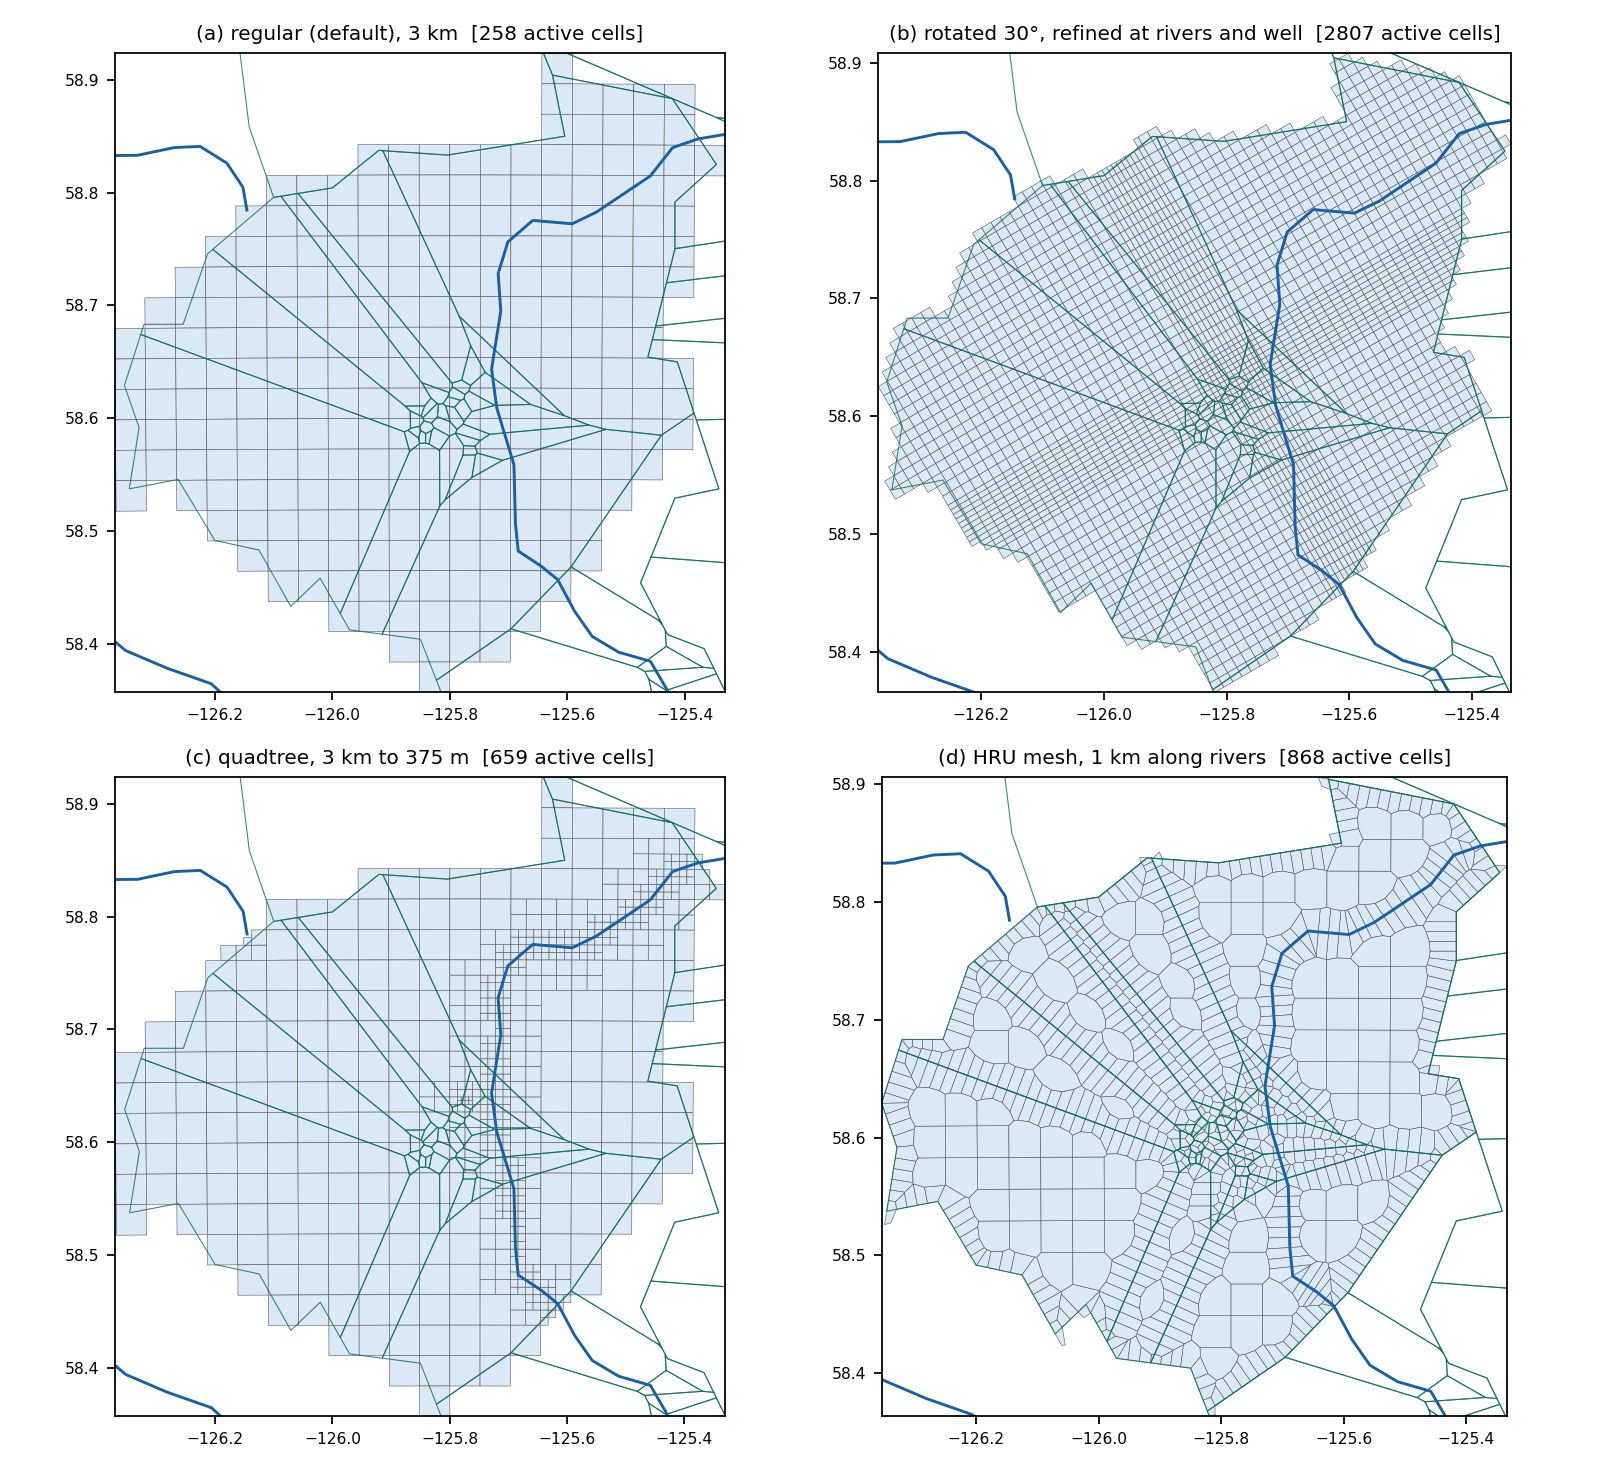
\includegraphics[width=0.78\linewidth]{figures/fig_grids.png}
\caption{The same model (Liard subbasin 52, HRU boundaries green, rivers blue) on four grids: (a) the default regular
grid; (b) rotated 30\textdegree{} and refined along rivers and around a well; (c) a quadtree refined along rivers and around the
well; (d) an HRU mesh whose cells follow HRU boundaries, with cells along the rivers.}\label{fig:grids}
\end{figure}

\subsection{Regular grids: rotation and variable spacing}
\cmd{:GridRotation} $\theta$ turns the grid $\theta$ degrees counterclockwise, for example to align columns with a valley.
The grid is built in its own rotated frame, in which every cell is still a rectangle; HRU polygons, rivers, wells and
boundaries are rotated into that frame, and MODFLOW receives the rotation as \cmd{ANGROT}. With \cmd{:GridRefinement} the grid gets variable spacing. Every base column and row that comes within the target size of a
refinement feature is divided into equal parts no larger than the target. Neighbouring columns and rows are then halved
until the widths change by at most a factor of two from one to the next. Refinement therefore always spans whole columns and rows.

\subsection{Quadtree grids}
A quadtree starts from large squares and cuts a square into four smaller ones wherever finer detail is wanted --- along a
river, say --- repeating until the cells are small enough. With \cmd{:GridType QUADTREE} a square is split into four while it is larger than the target size and a refinement feature
lies within half the target size of it. Splitting stops after \cmd{:QuadtreeMaxLevel} halvings (by default, enough to
reach the smallest target). The tree is then balanced so that neighbouring cells differ by one level at most. Where a large cell meets two
small ones its side carries the extra corner of the small cells (a hanging vertex), so MODFLOW's DISV input finds every
shared face. Because the line joining the centres of a large and a small cell is not perpendicular to their shared face,
MODFLOW's XT3D correction (the full conductance tensor) could be used. It is off by default, for two reasons found in the tests of Chapter~\ref{ch:verification}. The balanced quadtree was as
accurate without it (Thiem test). And XT3D --- even in its right-hand-side form --- slowed the Newton method badly where cells
dry and rewet: on the Liard model it took 32 instead of 7 iterations per day, and some days failed. \cmd{:FlowCorrection XT3D\_RHS} or \cmd{XT3D} switch it on.

\subsection{Meshes that follow HRU boundaries}
Picture a dot for every cell: each cell is the area closer to its own dot than to any other dot (a \emph{Voronoi} cell). If
two dots sit on opposite sides of an HRU boundary, at the same distance from it, the edge between their cells falls exactly
on that boundary. Raven places its dots this way, so the cells follow the HRU boundaries. In detail, with
\cmd{:GridType HRU\_MESH} the seed points are:
\begin{enumerate}
\item along every HRU boundary, pairs of seeds mirrored across the boundary at spacing $s_b=\min(\Delta/2,$ smallest
line refinement size (\cmd{RIVERS}, \cmd{LINES})$)$, or the \cmd{LAKES}/\cmd{POLYGONS} size where the boundary passes within
one such size of a refinement polygon, and $0.3\,s_b$ from it --- the face between the two seeds of a pair lies on the boundary;
\item seeds along refinement lines (rivers run through cell centres), in rings around refinement points (wells), and on a
staggered lattice of the target size inside and within one size around refinement polygons (lakes); seeds outside the
model's box (e.g.\ a monitoring well outside the model) are left out;
\item interior seeds on a lattice of spacing $\Delta$, kept only where no other seed is closer than about half the spacing.
\end{enumerate}
Each cell is the part of the plane closer to its seed than to any other. Raven builds it by cutting away, for each
neighbouring seed, the half of the plane that is closer to that neighbour. Each face remembers the seed on its other side, so
the connections between cells are exact. The line joining two seeds crosses their shared face at right angles, which is the
arrangement MODFLOW's standard method assumes, so no XT3D is needed. Where boundaries meet at sharp corners a cell may cover slivers of two HRUs. The overlaps are computed exactly, as for any
other grid, so the water accounts are unaffected. \cmd{GWModelSummary.txt} reports how much of each active cell's area lies
in its main HRU (typically above 99\%).

\subsection{Imported cells}
With \cmd{:GridType FILE} and \cmd{:GridFile cells.geojson ID\_FIELD} the cells are the polygons of a GeoJSON file in
longitude/latitude, one single-ring polygon per cell, numbered by the ID field (default \cmd{CELL\_ID}). Cells may be
concave, and a cell side may be shared with several smaller cells (T-junctions): neighbours are found wherever edges of two
cells lie on the same line --- within 0.1\% of the edge length, because a straight edge drawn in one map projection bends
slightly in another --- and overlap. A face made of several pieces gets their total length and their average position and
direction. Repeated vertices, which GIS exports often contain, are removed first. MODFLOW receives the grid as DISU with the
connection lengths, face widths and face directions computed from the polygons. Imported cells need not be orthogonal; for strongly non-orthogonal cells consider
\cmd{:FlowCorrection XT3D\_RHS} and check the convergence in \cmd{GWBudget.csv}.

\subsection{Connecting layers by elevation}
In a layered grid a cell connects sideways only to the cell with the same layer number. When neighbouring columns have
different profiles --- a gravel layer thinning out next to a till, say --- the same layer number can mean different
materials at different elevations. \cmd{:LayerConnection ELEVATION} writes the grid as DISU and connects every pair of
cells of neighbouring columns whose vertical intervals overlap, as staggered horizontal connections (MODFLOW's \cmd{IHC}
2), so water flows between the layers that actually touch. Pass-through cells are removed and the cells above and below
them connected directly.

\subsection{Refinement}
\begin{lstlisting}
:GridRefinement RIVERS   250                     # along :RiverGeometry lines
:GridRefinement WELLS    100                     # around pumping and monitoring wells
:GridRefinement LAKES    250                     # in and around every reservoir's lake HRU
:GridRefinement LINES    faults.geojson    200   # along any lines
:GridRefinement POLYGONS wetlands.geojson  250   # inside and around polygons
\end{lstlisting}
Sizes must be smaller than \cmd{:GridCellSize}. Refinement applies to regular (variable spacing), quadtree and HRU-mesh
grids; an imported grid is used as it is.

\cmd{LAKES} needs no extra file: the outline of the lake HRU of every Raven reservoir (\cmd{:Reservoir \dots\ :HRUID}) is taken
from \cmd{:HRUGeometry}. Fine cells around a lake place its seepage (\cmd{:ReservoirExchange}) and the exchange along its shore
more precisely. On a regular grid the rows and columns through the lake are refined; a quadtree splits the squares in and
near the lake; an HRU mesh places cells of the target size inside the lake and in a band one cell wide around it, and
shortens the spacing of its cells along the shore. \cmd{POLYGONS} works the same way for any outline in a file.

\subsection{Rivers and boundaries on any grid}
On the default grid river and boundary lines are cut into cells as before. On every other grid each piece of a line is cut exactly at the edges of the cells it crosses (rectangles along their
sides, other cells along their edges or triangle by triangle). River lengths per cell are therefore exact and do not
depend on the cell size. A stretch lying exactly on a shared cell edge
is counted once. A boundary line may be drawn along the edge of the modelled area, where the edge cells can be inactive because too little
of them is covered. Such a line is attached to the nearest active cell within one cell size, so a boundary drawn on the
watershed outline is never lost.

\subsection{Choosing a grid}
Start with the default grid and a cell size of a few kilometres. Refine where heads and exchanges change quickly: along
rivers that gain or lose much water, around pumping wells, around lakes and reservoirs that leak to the aquifer, and in
wetlands. A quadtree gives the most accuracy per cell;
an HRU mesh gives the cleanest HRU--cell linkage; a rotated regular grid is simplest when a valley has one direction. XT3D
(\cmd{:FlowCorrection XT3D\_RHS} or \cmd{XT3D}) is off by default; use it only for strongly non-orthogonal imported cells, and
check that the model still converges well.

\subsection{Grid outputs}
Every run writes \cmd{mf6/grid\_cells.geojson}: each cell as a longitude/latitude polygon with its number (as in MODFLOW and in
the hotstart file), whether it is active, its profile, its dominant HRU and its area --- ready to be joined with heads in
QGIS. For grids other than regular, \cmd{GWHeads.nc} has a \cmd{cell} dimension instead of rows and columns, and the hotstart
block is written as \cmd{:GWHeads} \emph{nlay} \cmd{1} \emph{ncells}. The grid type, cell sizes, MODFLOW format and HRU
fidelity are reported in \cmd{GWModelSummary.txt}. Setting the environment variable \cmd{RAVEN\_GW\_PROFILE=1} prints the time
taken by each stage of building the model, useful for large grids.

\section{Building the layers}\label{ch:layers}
\subsection{Land surface, model top and bedrock}
For each active column Raven needs three elevations:
\begin{description}
\item[Land surface] $z_{\mathrm{land},i}$: the average of 25 points ($5\times5$) of the DEM over the cell
(\cmd{:LandSurface}); without a DEM, the area-weighted \cmd{ELEVATION} of the HRUs in the cell.
\item[Model top] $z_{\mathrm{top},i}=z_{\mathrm{land},i}-d_{\mathrm{sz},p}$, where $d_{\mathrm{sz}}$ is the profile's
\cmd{SOIL\_ZONE\_DEPTH} (default 0, so the top is the land surface).
\item[Bedrock] $z_{\mathrm{br},i}$: the average of 25 points of the bedrock map (\cmd{:BedrockSurface}); without a map,
$z_{\mathrm{land},i}-D_p$ with $D_p$ the profile's \cmd{DEFAULT\_BEDROCK\_DEPTH}.
\end{description}
A column whose bedrock lies less than 0.5 m below its top has no room for an aquifer and is made inactive.

\subsection{Stacking the layers}
A profile lists its layers from the top down, each with a material (\emph{aquifer class}), a thickness $b_\ell$ (or
\cmd{TO\_BEDROCK}) and a type. The bottom of layer $\ell$ is
\begin{equation}
z^{(\ell)}_{\mathrm{bot},i}=
\begin{cases}
z_{\mathrm{br},i} & \text{for a \cmd{TO\_BEDROCK} layer,}\\
\max\!\left(z^{(\ell-1)}_{\mathrm{bot},i}-b_\ell,\;z_{\mathrm{br},i}\right) & \text{otherwise,}
\end{cases}
\qquad z^{(0)}_{\mathrm{bot},i}\equiv z_{\mathrm{top},i}.
\end{equation}
Layers never extend below bedrock. Two special cases:
\begin{itemize}
\item A layer (other than the first) cut to less than 0.5 m by bedrock becomes a \emph{pass-through} cell: it is given
a nominal thickness of 0.01 m and MODFLOW's \cmd{IDOMAIN}~$=-1$, which removes it from the calculation while
connecting the cells above and below it directly.
\item The model has as many layers as the thickest profile. Where a profile has fewer layers, the missing ones are
pass-through cells.
\end{itemize}

\begin{example}[: one column]
Land surface 600 m, bedrock 555 m, profile \cmd{VALLEY\_ALLUVIUM} = gravel 15 m, clay till 5 m, sand \cmd{TO\_BEDROCK}.
Top = 600 m. Layer 1 (gravel): bottom $\max(600-15,555)=585$ m. Layer 2 (till): bottom $\max(585-5,555)=580$ m.
Layer 3 (sand): bottom 555 m (to bedrock), thickness 25 m. If bedrock were at 582 m instead, layer 2 would end at
$\max(580,582)=582$ m (3 m thick), and layer 3, which runs to bedrock, would span 582 to 582 m --- zero thickness, so it becomes
a pass-through cell.
\end{example}

\begin{figure}[!htbp]\centering
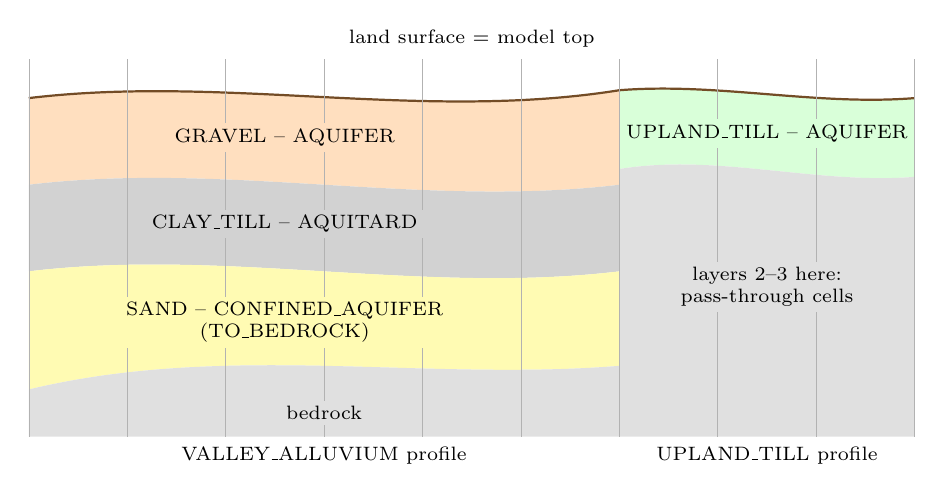
\begin{tikzpicture}[x=1.25cm,y=1.0cm,lab/.style={font=\scriptsize,align=center,inner sep=2pt}]
\fill[orange!25] (0,4.3) .. controls (2,4.6) and (4,4.0) .. (6,4.4) -- (6,3.2) .. controls (4,2.9) and (2,3.5) .. (0,3.2) -- cycle;
\fill[gray!35] (0,3.2) .. controls (2,3.5) and (4,2.9) .. (6,3.2) -- (6,2.1) .. controls (4,1.8) and (2,2.4) .. (0,2.1) -- cycle;
\fill[yellow!30] (0,2.1) .. controls (2,2.4) and (4,1.8) .. (6,2.1) -- (6,0.9) .. controls (4,0.7) and (2,1.2) .. (0,0.6) -- cycle;
\fill[black!12] (0,0.6) .. controls (2,1.2) and (4,0.7) .. (6,0.9) -- (6,0) -- (0,0) -- cycle;
\fill[green!15] (6,4.4) .. controls (7,4.5) and (8,4.2) .. (9,4.3) -- (9,3.3) .. controls (8,3.2) and (7,3.6) .. (6,3.4) -- cycle;
\fill[black!12] (6,0) -- (6,3.4) .. controls (7,3.6) and (8,3.2) .. (9,3.3) -- (9,0) -- cycle;
\draw[thick,brown!60!black] (0,4.3) .. controls (2,4.6) and (4,4.0) .. (6,4.4) .. controls (7,4.5) and (8,4.2) .. (9,4.3);
\foreach \x in {0,1,...,9} \draw[gray!60,very thin] (\x,0) -- (\x,4.8);
\node[lab,fill=white,inner sep=1pt] at (4.5,5.05) {land surface = model top};
\node[lab,fill=orange!25] at (2.6,3.8) {GRAVEL -- \cmd{AQUIFER}};
\node[lab,fill=gray!35] at (2.6,2.7) {CLAY\_TILL -- \cmd{AQUITARD}};
\node[lab,fill=yellow!30] at (2.6,1.45) {SAND -- \cmd{CONFINED\_AQUIFER}\\ (\cmd{TO\_BEDROCK})};
\node[lab,fill=black!12] at (3.0,0.3) {bedrock};
\node[lab,fill=green!15] at (7.5,3.85) {UPLAND\_TILL -- \cmd{AQUIFER}};
\node[lab,fill=black!12] at (7.5,1.9) {layers 2--3 here:\\ pass-through cells};
\node[lab,anchor=north] at (3,-0.05) {\cmd{VALLEY\_ALLUVIUM} profile};
\node[lab,anchor=north] at (7.5,-0.05) {\cmd{UPLAND\_TILL} profile};
\end{tikzpicture}
\caption{Layers are stacked from the model top and clipped at bedrock; the one-layer upland profile is padded with
pass-through cells.}\label{fig:layers}
\end{figure}

\subsection{Layer types}
\begin{table}[!htbp]\centering
\caption{Layer types.}\label{tab:types}\small
\begin{tabular}{P{0.31\linewidth}P{0.27\linewidth}P{0.348\linewidth}}\toprule\hdr
Type in the profile & MODFLOW 6 setting & What it means\\\midrule
\cmd{AQUIFER} (\cmd{UNCONFINED\_AQUIFER}) & \cmd{ICELLTYPE}=1, \cmd{ICONVERT}=1 & water table can be inside the layer: storage by $S_y$, transmissivity from the saturated thickness\\
\cmd{CONFINED\_AQUIFER} & \cmd{ICELLTYPE}=0, \cmd{ICONVERT}=0 & always full: constant transmissivity, storage by $S_s$\\
\cmd{AQUITARD}, \cmd{CONFINING\_LAYER} & as \cmd{AQUIFER}, with the low $K$ of its class & slow leaky layer, simulated explicitly\\
\cmd{AQUICLUDE} & \cmd{IDOMAIN}=0 & no flow at all through this layer (not allowed as the top layer)\\\bottomrule
\end{tabular}
\end{table}

\subsection{Material properties}
Each layer takes its properties from its aquifer class (\cmd{:AquiferClasses}): horizontal conductivity $K_h$
(\cmd{K\_HORIZ}), vertical conductivity $K_v$ (\cmd{K\_VERT}, default $K_h/10$), $S_s$ (\cmd{SPEC\_STORAGE}, default
$10^{-5}$), $S_y$ (\cmd{SPEC\_YIELD}, default 0.1) and porosity (\cmd{POROSITY}, default 0.3; stored for future transport
calculations; MODFLOW's flow calculation does not use it).

\begin{watch}
MODFLOW connects layer $\ell$ of one column sideways only to layer $\ell$ of its neighbours. Where two profiles meet,
list their layers in the same geological order, otherwise, for example, a gravel layer may connect to a clay layer.
\end{watch}

\subsection{Initial heads}
The starting head of every cell in a column is
\begin{equation}
h^0_i=\max\!\left(z_{\mathrm{land},i}-d_0,\;z_{\mathrm{low},i}+0.1\right),
\end{equation}
where $d_0$ is the profile's \cmd{INITIAL\_HEAD\_DEPTH} (or the value given by \cmd{:InitialGWHeads} in the \cmd{.rvc}
file), and $z_{\mathrm{low},i}$ is the bottom of the lowest active cell. With \cmd{:InitialGWHeads ELEVATION z}, $z$ replaces $z_{\mathrm{land},i}-d_0$ (still at least 0.1 m above the lowest active cell bottom).
A hotstart (\cmd{:GWHeads} in the \cmd{.rvc}) overrides all of this cell by cell. Optionally, a steady-state
calculation replaces these first guesses (Section~\ref{sec:init}).

\subsection{The generated MODFLOW files}
Raven writes a standard MODFLOW~6 simulation to \cmd{<output>/mf6/}: \cmd{mfsim.nam} (simulation), \cmd{sim.tdis}
(time steps), \cmd{sim.ims} (solver), \cmd{gwf.nam} (model), \cmd{gwf.dis} (grid), \cmd{gwf.npf} (conductivities and
layer types), \cmd{gwf.sto} (storage), \cmd{gwf.ic} (initial heads), \cmd{gwf.oc} (output control) and one file per
exchange package (\cmd{gwf.rch}, \cmd{gwf.drn}, \cmd{gwf.riv}, \cmd{gwf.evt}, \cmd{gwf.wel}, \cmd{gwf.ghb}, \cmd{gwf.chd},
\cmd{gwf.swx}, \cmd{gwf.res}). Grid arrays are written layer by layer, each grid row starting on a new line, which is
how MODFLOW reads them. These files can be opened in FloPy or ModelMuse; they never need editing.

\section{Parameters used to build the model}\label{sec:buildparams}
The grid and layers are built from the following parameters; the class column says where each is set, the reference column
where its default and allowed range are listed.
\begin{table}[!htbp]\centering
\caption{Parameters used to build the model.}
\begin{tabular}{>{\raggedright\arraybackslash}P{0.09\linewidth}>{\raggedright\arraybackslash}P{0.26\linewidth}>{\raggedright\arraybackslash}P{0.287\linewidth}>{\raggedright\arraybackslash}P{0.1\linewidth}>{\raggedright\arraybackslash}P{0.15\linewidth}}\toprule\hdr
Symbol & Parameter & Class (where it is set) & Units & Reference\\\midrule
$\Delta$ & \cmd{:GridCellSize} & \cmd{.rvg} option & m & Sec.~\ref{app:commands}\\
$f_{\min}$ & \cmd{:MinCellCoverage} & \cmd{.rvg} option & -- & Sec.~\ref{app:commands}\\
-- & \cmd{AQUIFER\_PROFILE} & HRU attribute (\cmd{:HRUs}, \cmd{.rvh}) & -- & Sec.~\ref{app:commands}\\
$P_k$ & HRU polygon & \cmd{:HRUGeometry} (\cmd{.rvg}) & -- & Sec.~\ref{app:commands}\\
$z_{\mathrm{land}}$ & land surface & \cmd{:LandSurface} (\cmd{.rvg}); else HRU \cmd{ELEVATION} & m & Sec.~\ref{app:commands}\\
$z_{\mathrm{br}}$ & bedrock & \cmd{:BedrockSurface} (\cmd{.rvg}); else \cmd{DEFAULT\_BEDROCK\_DEPTH} (aquifer profile) & m & Sec.~\ref{app:profile}\\
$d_{\mathrm{sz}}$ & \cmd{SOIL\_ZONE\_DEPTH} & aquifer profile & m & Sec.~\ref{app:profile}\\
$b_\ell$ & layer thickness, type & aquifer profile (\cmd{:AquiferProfiles}) & m & Sec.~\ref{app:layers}\\
$K_h$, $K_v$ & \cmd{K\_HORIZ}, \cmd{K\_VERT} & aquifer class of the layer & m/d & Sec.~\ref{app:class}\\
$S_s$, $S_y$ & \cmd{SPEC\_STORAGE}, \cmd{SPEC\_YIELD} & aquifer class of the layer & 1/m, -- & Sec.~\ref{app:class}\\
$d_0$ & \cmd{INITIAL\_HEAD\_DEPTH}; \cmd{:InitialGWHeads} & aquifer profile; \cmd{.rvc} & m & Sec.~\ref{app:profile}\\
\bottomrule
\end{tabular}
\end{table}

\section{What the generated files look like}
The model name file lists the packages Raven uses:
\begin{lstlisting}
BEGIN OPTIONS
  NEWTON
END OPTIONS
BEGIN PACKAGES
  DIS6  gwf.dis  DIS
  NPF6  gwf.npf  NPF
  STO6  gwf.sto  STO
  IC6   gwf.ic   IC
  RCH6  gwf.rch  RCH_RAVEN
  DRN6  gwf.drn  DRN_RAVEN
  RIV6  gwf.riv  RIV_RAVEN
  OC6   gwf.oc   OC
END PACKAGES
\end{lstlisting}
The grid file records the projection in its first line, so the grid can be placed on a map:
\par\noindent\begin{minipage}{\linewidth}
\begin{lstlisting}
# Lambert azimuthal equal-area projection, origin lat=58.81662353 lon=-125.4914706 (sphere R=6371007.181 m)
BEGIN DIMENSIONS
  NLAY 3
  NROW 85
  NCOL 54
END DIMENSIONS
\end{lstlisting}
\end{minipage}\par\smallskip
Boundary packages contain one line per cell with placeholder values; Raven replaces the values in memory every step, so
the files show the grid positions of recharge, drains, rivers, wells and boundaries but not their daily values.

\section{Solver settings}
Why such a small head tolerance? MODFLOW stops iterating when no head changes by more than the tolerance, but a flow is a
conductance times a head difference. The seepage drains have very large conductances (one 1 km cell with a leakance of
1~d$^{-1}$ has $10^6$~m$^2$/d), so a head tolerance of 1 cm could still leave about $10^4$~m$^3$/d of imbalance in such a cell on a
difficult day. With 0.01 mm the imbalance is a thousand times smaller than with 1 cm. The price is more Newton iterations --- in the
20-year Liard run about 10 per day on average instead of 7--8 --- and a longer run (about 15 instead of 8 minutes). The value was chosen from the
randomized tests: at 0.1 mm a few extreme set-ups (drain conductance $2\times10^7$~m$^2$/d per cell) still showed a 0.2\%
residual on single steps; at 0.01 mm none did.

\paragraph{Two-tier convergence.} A very tight tolerance can occasionally stall the Newton iterations on a hard step. The target is the tolerance above. If a step has not reached it after 100 iterations (or half the iteration limit, if that is smaller), the coupler raises
MODFLOW's own tolerance to ten times the target (0.1 mm) for the rest of that step only, and restores it for the next step. MODFLOW's own test always decides whether a step has converged. A step accepted at the relaxed tolerance is therefore as
reliable as a step of a model run with that tolerance. Only if even that fails within the iteration limit is the step
reported as not converged. \cmd{GWBudget.csv} records which
case applied (\emph{converged} = 1 target reached, 2 accepted at the relaxed tolerance, 0 not converged).
The water exchanged between Raven and MODFLOW is exact at any tolerance --- both sides use the same computed flows ---
so the tolerance only controls MODFLOW's own small numerical residual.

\begin{table}[!htbp]\centering
\caption{MODFLOW solver settings (\cmd{sim.ims}).}
\begin{tabular}{P{0.36\linewidth}P{0.14\linewidth}P{0.428\linewidth}}\toprule\hdr
IMS setting & Value & Meaning\\\midrule
\cmd{COMPLEXITY} & \cmd{COMPLEX} & robust defaults for non-linear problems\\
\cmd{OUTER\_DVCLOSE} & 0.00001 m & Newton iterations stop when no head changes by more than this (\cmd{:SolverHead\allowbreak Tolerance})\\
\cmd{OUTER\_MAXIMUM} & 500 & iteration limit (\cmd{:SolverMax\allowbreak OuterIterations})\\
\cmd{UNDER\_RELAXATION} & \cmd{DBD} & damps oscillating head changes (theta 0.7, kappa 0.07, gamma 0.1)\\
\cmd{BACKTRACKING\_NUMBER} & 20 & retries with a smaller step when the imbalance grows\\
\cmd{INNER\_MAXIMUM} & 500 & linear-solver iteration limit\\
\cmd{INNER\_DVCLOSE}, \cmd{INNER\_RCLOSE} & $0.1\times$ outer, 1 m$^3$/d & linear-solver tolerances\\
\cmd{LINEAR\_ACCELERATION} & \cmd{BICGSTAB} & linear solver\\
\cmd{PRECONDITIONER\_LEVELS} & 5 & ILU fill level\\\bottomrule
\end{tabular}
\end{table}

\section{How MODFLOW solves each time step}\label{ch:mf6}
\subsection{Time steps}
MODFLOW's time steps are generated from Raven's \cmd{:StartDate}, \cmd{:Duration} and \cmd{:TimeStep}: one transient
stress period of $N=\mathrm{round}(T/\dt)$ steps of length $\dt$, preceded by a one-day steady-state period when
\cmd{:GWInitialization STEADY\_STATE} is used. MODFLOW therefore always takes exactly one step for each Raven step.
If Raven would run more steps than MODFLOW holds, Raven stops with a clear message.

\subsection{Cells that dry and rewet: the Newton method}
An unconfined cell whose water table falls below its bottom is \emph{dry}. Older MODFLOW versions switched such cells
off, which often made the solution fail when they needed to switch back on. MODFLOW~6's Newton--Raphson method, which the coupling always uses, keeps dry cells in the calculation. The conductance
between two cells is scaled smoothly by how full the upstream cell is, and falls to zero as that cell empties. The cell
fills again naturally when water arrives. The solver settings written by Raven are:
\begin{itemize}
\item outer (Newton) iterations up to 500 (\cmd{:SolverMax\allowbreak OuterIterations}), head-change tolerance 0.00001 m (\cmd{:SolverHead\allowbreak Tolerance});
\item delta-bar-delta under-relaxation (damps oscillating head changes) and backtracking (retries a smaller change
when the residual grows);
\item inner linear solver BiCGSTAB with an ILU preconditioner of level 5, residual tolerance 1.0 m$^3$/d.
\end{itemize}
The Newton option is written without its own \cmd{UNDER\_RELAXATION} keyword, which resets a head that falls below the cell
bottom. With MODFLOW~6.6 that reset made the Newton change of a drying cell repeat unchanged at every iteration, so the
step never converged (on the Liard model this happened on most days once the thin aquitard under the gravel began to dry).
Without it, MODFLOW~6.6.3 and 6.8.1 converge in the same few iterations.
Raven runs the Newton iterations itself through MODFLOW's interface (prepare, repeated solve, finalize), so it knows
whether each step converged. If a step does not converge, MODFLOW continues (option \cmd{CONTINUE}), the step is
flagged in \cmd{GWBudget.csv}, and a safeguard limits what that step can return to Raven (Section~\ref{sec:guard}).

\subsection{Connectivity between aquifer areas}
Because dry cells carry no flow, parts of an aquifer can become disconnected when the water table falls and join
again when it rises, without any action by the user. Streams disconnect from a falling water table in the same way
(Section~\ref{ch:rivers}). To show this, \cmd{GWConnectivity.csv} reports each step:
\begin{itemize}
\item the fraction of top-layer cells of each profile that are \emph{wet}, meaning $h_i>z^{(1)}_{\mathrm{bot},i}+10^{-3}$ m;
\item the number of separate wet areas, where two wet cells belong to the same area if they share an edge
(4-neighbour connectivity; counted by a flood-fill of the wet cells).
\end{itemize}
This is a diagnostic only; it does not affect the calculation.

\subsection{Heads of dry cells}
Under the Newton method a dry cell carries no flow, and MODFLOW leaves its head at whatever value the solver reaches; it
can be far below the cell bottom (values of $-10^{8}$~m have been seen in a pumped, isolated cell). MODFLOW's own flows are
unaffected, but such a head is not a water level. Wherever the coupling needs a real water level it therefore uses the \emph{water table} of the column: the head of the
highest cell whose head is above its bottom, or the bottom of the lowest active cell if all are dry. This is used for the
reservoir's local groundwater level, in \cmd{GWHRUState.csv}, and for monitoring wells (a well screened in a dry cell
reports a missing value, \cmd{-1.2345}). The MODFLOW head file and the hotstart heads keep
MODFLOW's raw values, so a restart continues exactly.
